
\documentclass[12pt]{article}
\usepackage{graphicx}
\usepackage{amsmath}
\usepackage{mathtools}
\usepackage{gensymb}
\usepackage{tabularx}
\usepackage{array}
\usepackage[latin1]{inputenc}
\usepackage{fullpage}
\usepackage{color}
\usepackage{array}
\usepackage{longtable}
\usepackage{calc}
\usepackage{multirow}
\usepackage{hhline}
\usepackage{ifthen}
\usepackage{lscape}
\usepackage{float}
\usepackage{amssymb}

\newcommand{\mydet}[1]{\ensuremath{\begin{vmatrix}#1\end{vmatrix}}}
\providecommand{\brak}[1]{\ensuremath{\left(#1\right)}}
\providecommand{\norm}[1]{\left\lVert#1\right\rVert}
\providecommand{\abs}[1]{\left\vert#1\right\vert}
\newcommand{\solution}{\noindent \textbf{Solution: }}
\newcommand{\myvec}[1]{\ensuremath{\begin{pmatrix}#1\end{pmatrix}}}
\let\vec\mathbf

\def\inputGnumericTable{}

\begin{document}
\begin{center}
\textbf\large{OPTIMIZATION}

\end{center}
\section*{Excercise 6.6}

Q4. Find the equation of normal to the curve $x^2=4y$ which passes through the point (4,-2)

\solution
The given equation of the curve can be written as  
\begin{align}
	\label{eq:parabolaEq2}
	g\brak{\vec{x}} = \vec{x}^T\vec{V}\vec{x} + 2\vec{u}^T\vec{x} + f = 0 
\end{align}
where
\begin{align}
	\label{eq:eqV}
	\vec{V} &= \myvec{ 1 & 0 \\ 0 & 0} \\
	\label{eq:eqU}
	\vec{u} &= \myvec{0 \\ -2} \\
	\label{eq:eqF}
	f &= 0 
\end{align}
We are given that 
\begin{align}
	\vec{h} &= \myvec{4 \\ -2}
\end{align}
This can be formulated as optimization problem as below:
\begin{align}
	\label{eq:Eq3}
	&  \min_{\vec{x}} \quad \text{f}\brak{\vec{x}} = \norm{\vec{x}-\vec{h}}^2\\
	\label{eq:Eq4}
	& \text{s.t.}\quad g\brak{\vec{x}} = \vec{x}^T\vec{V}\vec{x} + 2\vec{u}^T\vec{x} + f = 0  
\end{align}
It is already proved that the optimization problem is non-convex. However, by relaxing the constraint in \eqref{eq:Eq4} as
\begin{align}
	\label{eq:Eq7}
	& g\brak{\vec{x}} = \vec{x}^\top\vec{V}\vec{x} + 2\vec{u}^\top\vec{x} + f \le 0  
\end{align}
the optimization problem can be made convex.
We will use Lagrange multipliers method to find the optimum value. Define
\begin{align}
	H\brak{\vec{x}, \lambda} &= f\brak{\vec{x}} - \lambda g\brak{\vec{x}} 
\end{align}
and we find that 
\begin{align}
	\nabla f\brak{\vec{x}} &= 2\brak{\vec{x}-\vec{h}} \\
	\nabla g\brak{\vec{x}} &= 2\brak{\vec{V}\vec{x}+\vec{u}}
\end{align}
We have to find $\lambda \in \mathbb{R}$ such that
\begin{align}
	&\nabla H\brak{\vec{x},\lambda} = 0 \\
        \label{eq:Eqlambda}
	&\implies 2\brak{\vec{x}-\vec{h}} - 2\lambda\brak{\vec{V}\vec{x}+\vec{u}} = 0 \\
        \label{eq:Eqx}
	&\implies \vec{x} - \vec{h} =  \lambda\brak{\vec{V}\vec{x}+\vec{u}}   \\
	&\implies \brak{\vec{I} - \lambda\vec{V}}\vec{x} =  \lambda\vec{u}+\vec{h} \\ 
	&\implies \myvec{1-\lambda & 0 \\ 0 & 1}\vec{x} = \lambda\myvec{0 \\ -2} + \myvec{4 \\-2} \\ 
        \label{eq:EqL}
	&\implies \myvec{1-\lambda & 0 \\ 0 & 1}\vec{x} = \myvec{4 \\ -2\lambda-2}  
\end{align}
Writing augmented matrix,
\begin{align}
	&\myvec{1-\lambda & 0 & 4\\ 0 & 1 & -2\lambda-2} \xleftrightarrow[]{R_1 \leftarrow \frac{R_1}{1-\lambda}} \myvec{1&0&\frac{4}{1-\lambda}\\0&1&-2\lambda-2}
\end{align}
Then, we get
\begin{align}
        \label{eq:Eqxm}
	\vec{x}_{m} &= \myvec{ \frac{4}{1-\lambda} \\ -2\lambda-2}
\end{align}
Substituting this value in \eqref{eq:Eq4}
\begin{align}
	\myvec{\frac{4}{1-\lambda}&-2-2\lambda}\myvec{1&0\\0&0}\myvec{\frac{4}{1-\lambda}\\-2-2\lambda}+2\myvec{0&-2}\myvec{\frac{4}{1-\lambda}\\-2-2\lambda} &= 0\\
	\frac{16}{\brak{1-\lambda}^2}+8\brak{\lambda+1} &= 0\\
	\lambda^3-\lambda^2-\lambda+3&=0\\
	\implies \lambda &= -1.3593
\end{align}
Substituting the value of $\lambda$ in \eqref{eq:Eqxm}
\begin{align}
	\vec{x}_{m} = \myvec{1.695\\0.718}
\end{align}
See figure \ref{fig:Fig1}
\begin{figure}[!h]
	\begin{center} 
	    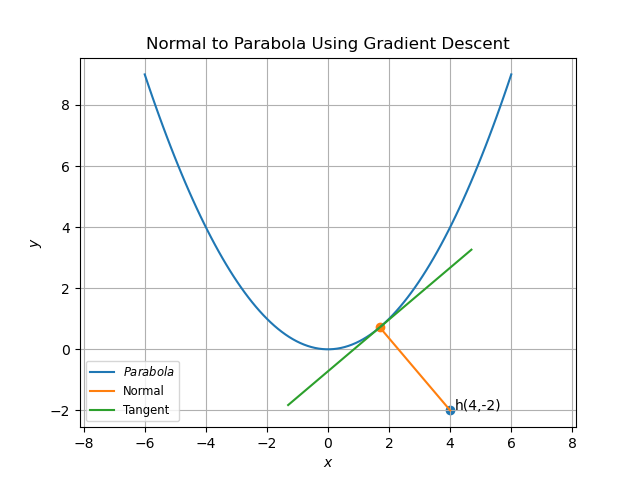
\includegraphics[width=\columnwidth]{figs/12_6_6_4_lagrange}
	\end{center}
\caption{}
\label{fig:Fig1}
\end{figure}
\end{document}
